\documentclass{beamer}
\usetheme{Berlin}
\usepackage[utf8]{inputenc}
\usepackage{amsmath,amssymb,graphicx,changepage,xcolor}

\newcommand{\Beta}{\textrm{Beta}}
\newcommand{\Bern}{\textrm{Bern}}
\newcommand{\Bin}{\textrm{Bin}}
\newcommand{\Expo}{\textrm{Expo}}
\newcommand{\Unif}{\textrm{Unif}}
\newcommand{\Pois}{\textrm{Pois}}
\newcommand{\Normal}{\mathcal{N}}
\newcommand{\NBin}{\textrm{NBin}}
\newcommand{\Geom}{\textrm{Geom}}
\newcommand{\FS}{\textrm{FS}}
\newcommand{\HGeom}{\textrm{HGeom}}
\newcommand{\Cauchy}{\textrm{Cauchy}}
\newcommand{\Logistic}{\textrm{Logistic}}
\newcommand{\Laplace}{\textrm{Laplace}}
\newcommand{\GammaDist}{\textrm{Gamma}}
\newcommand{\Corr}{\textrm{Corr}}
\newcommand{\Cov}{\textrm{Cov}}
\newcommand{\Var}{\textrm{Var}}
\newcommand{\SD}{\textrm{SD}}
\newcommand{\indep}{\perp \!\!\! \perp}
\newcommand{\B}{\boldsymbol}
\newcommand{\borel}{\mathcal{B}}
\newcommand{\Borel}{\mathcal{B}(\mathbb{R})}
\newcommand{\filt}{\mathcal{F}}
\newcommand{\ind}{\mathbb{I}}
\newcommand{\E}{\mathbb{E}}
\newcommand{\Prob}{\mathbb{P}}
\newcommand{\Est}{\textsc{est}}
\newcommand{\Stop}{\textsc{stop}}
\newcommand{\ceil}[1]{\left\lceil #1 \right\rceil}
\newcommand{\eps}{\varepsilon}

\title{Estimating Graph Parameters with Random Walks}
\subtitle{Anna Ben-Hamou, Roberto I. Oliveira, and Yuval Peres}
\author{Max L., Eric S, and Ivan S.}
\institute{Stat 212}
\date{April 27, 2022}

\begin{document}

\begin{frame}
\titlepage
\end{frame}

\begin{frame}
\frametitle{Contents}
\tableofcontents
\end{frame}

%%%%%%%%%%

\section{Introduction and Setup}
\subsection{Motivation}
\begin{frame}
\frametitle{Premise}
Consider a fixed (non-random) graph $G=(V,E)$, with $|V|=n$ vertices (nodes) and $|E|=m$ edges.\medskip

We don't know $G$ in advance: it could possibly have millions to billions of vertices or edges.\medskip

Consider \textbf{lazy random walks} (\textsc{lrw}s) on $G$, starting from the same vertex $x$: with probability $\frac{1}{2}$ we stay at the current vertex; otherwise we move to a neighbor with uniform probability.
\end{frame}

\begin{frame}
\frametitle{Toy Example}
\begin{figure}
    \centering
    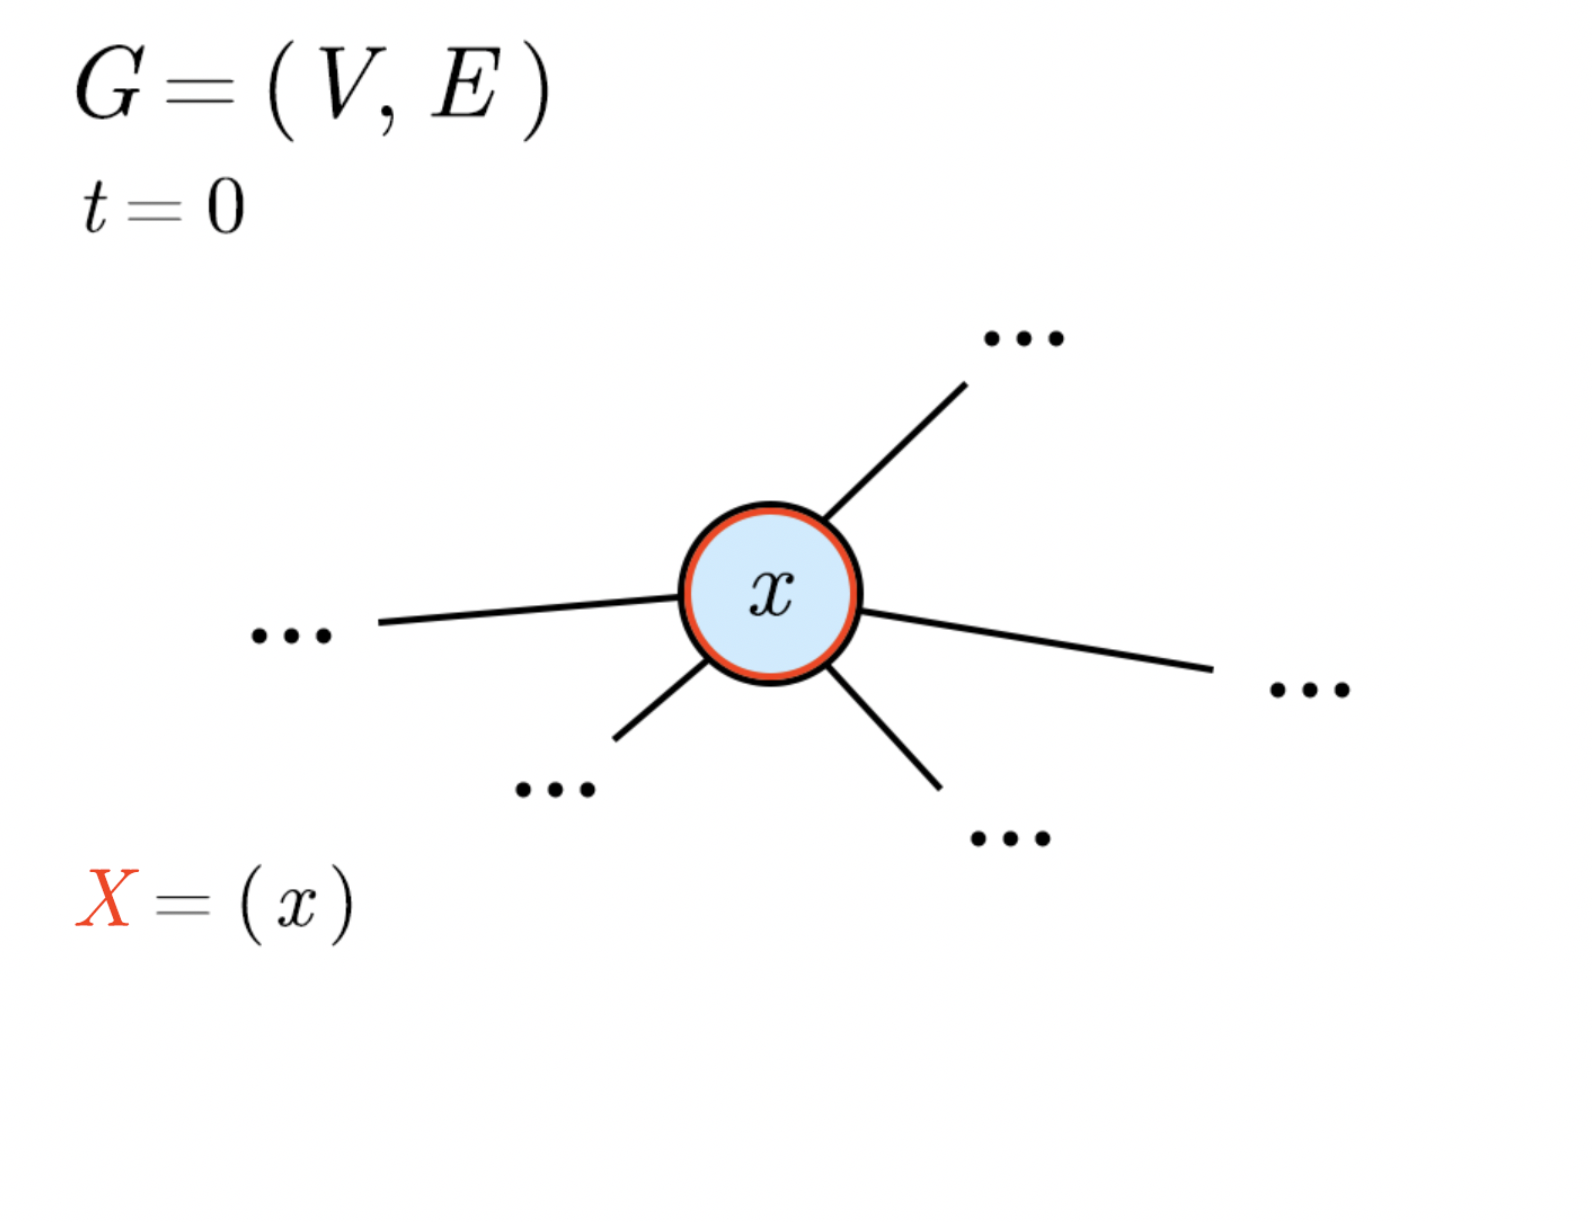
\includegraphics[trim={0 2cm 0 0}, clip, width=8cm]{diagrams/1.png}
\end{figure}
\end{frame}

\begin{frame}
\frametitle{Toy Example}
\begin{figure}
    \centering
    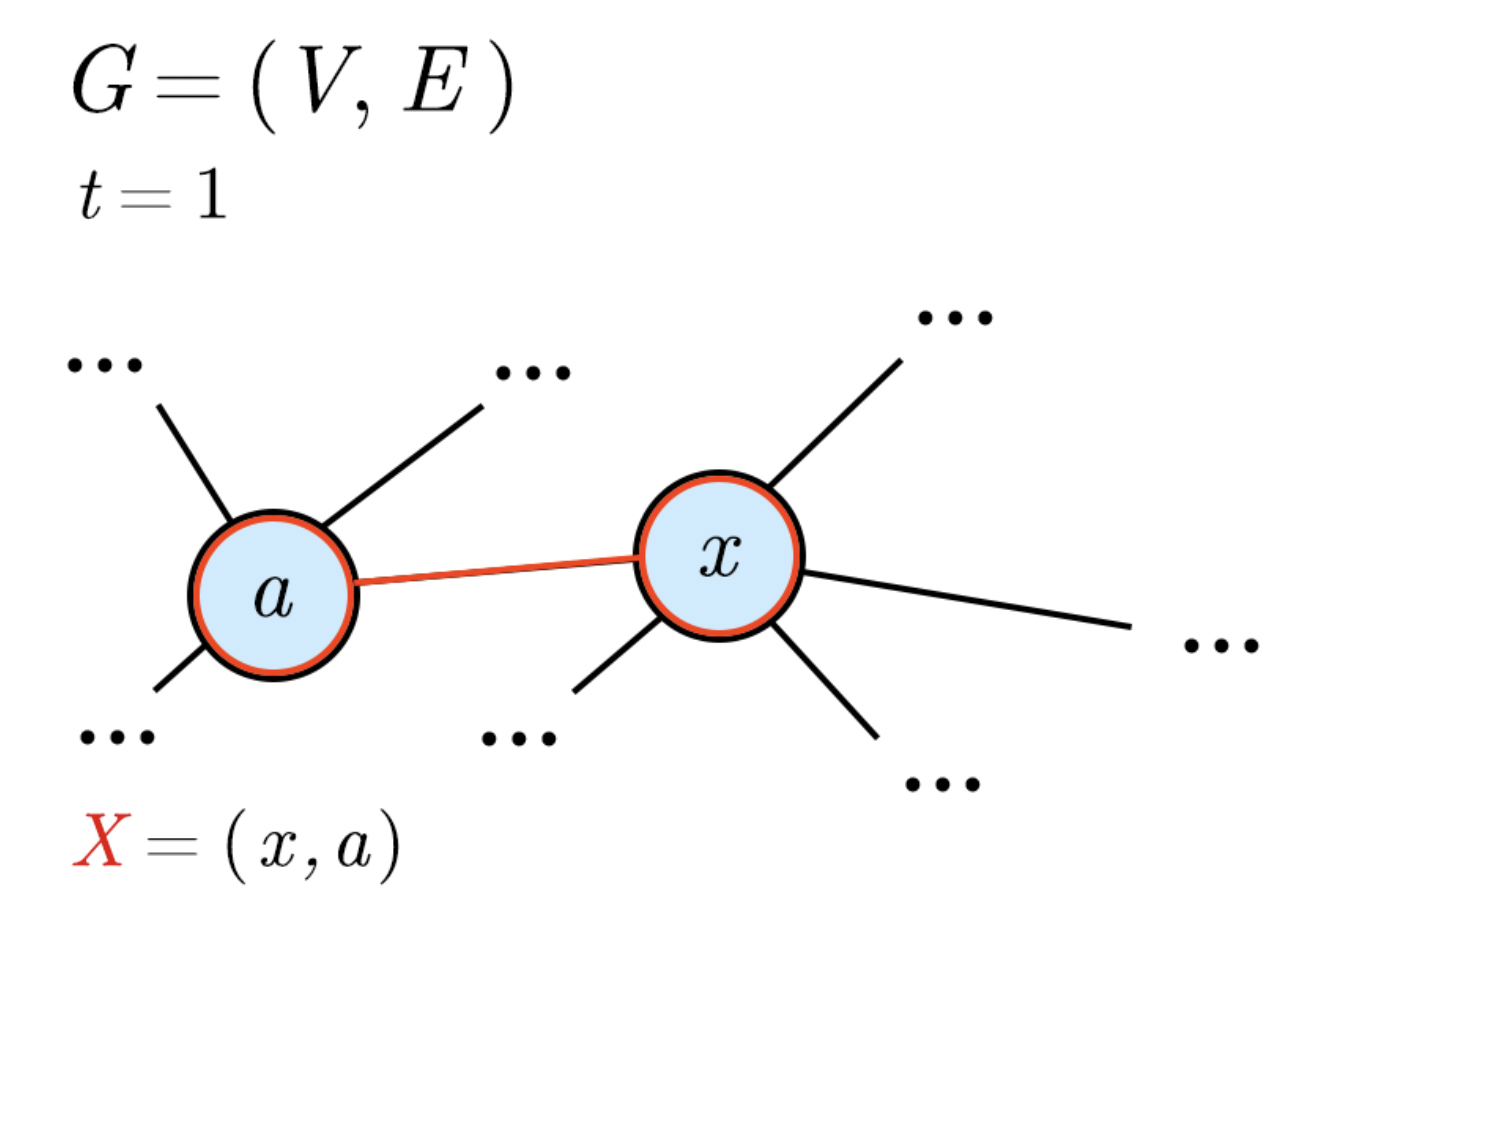
\includegraphics[trim={0 2cm 0 0}, clip, width=8cm]{diagrams/2.png}
\end{figure}
\end{frame}

\begin{frame}
\frametitle{Toy Example}
\begin{figure}
    \centering
    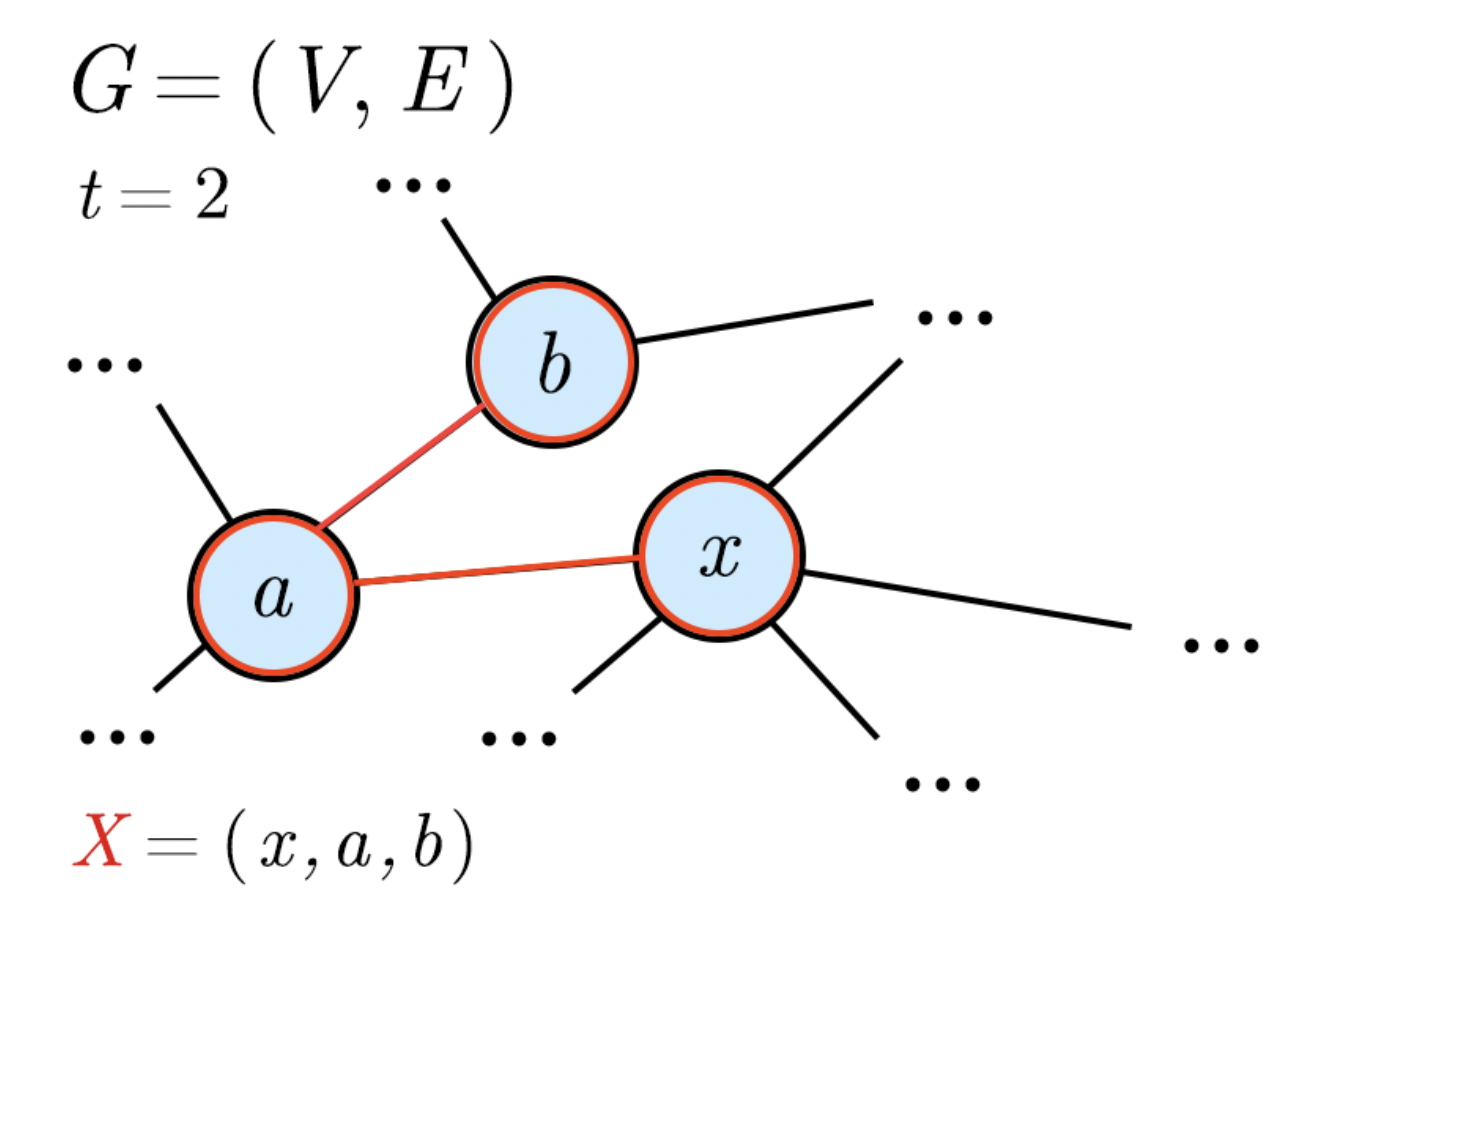
\includegraphics[trim={0 2cm 0 0}, clip, width=8cm]{diagrams/3.png}
\end{figure}
\end{frame}

\begin{frame}
\frametitle{Toy Example}
\begin{figure}
    \centering
    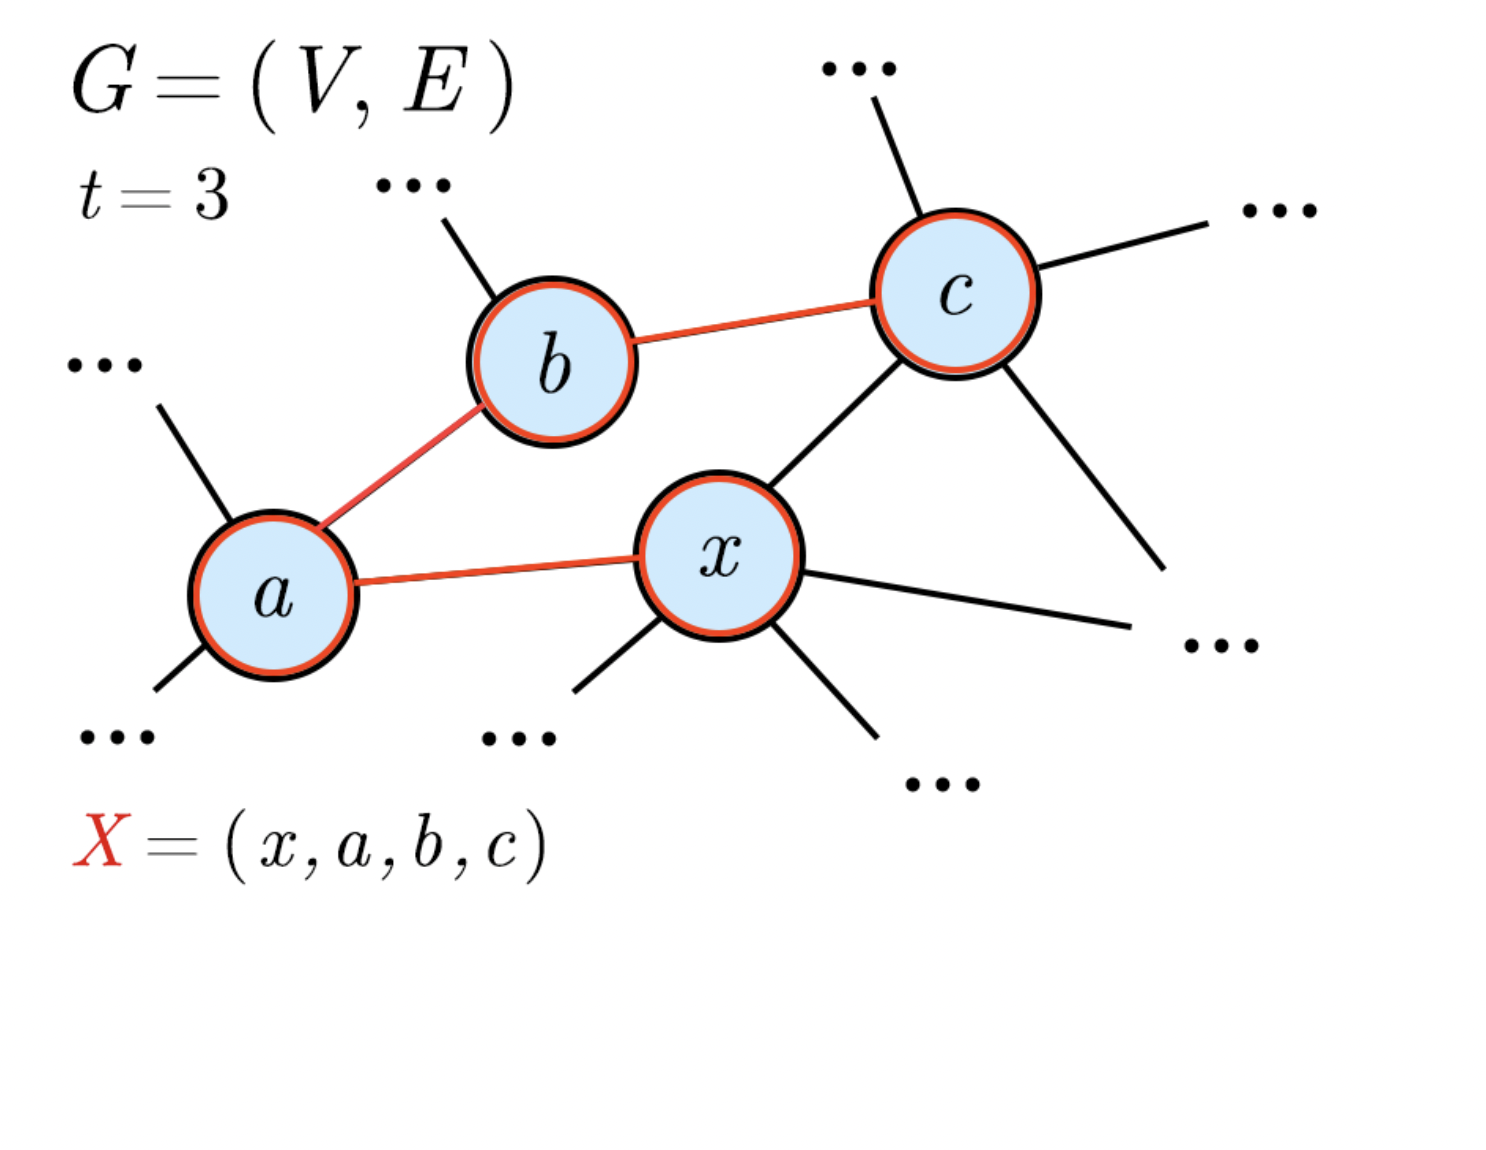
\includegraphics[trim={0 2cm 0 0}, clip, width=8cm]{diagrams/4.png}
\end{figure}
\end{frame}

\begin{frame}
\frametitle{Toy Example}
\begin{figure}
    \centering
    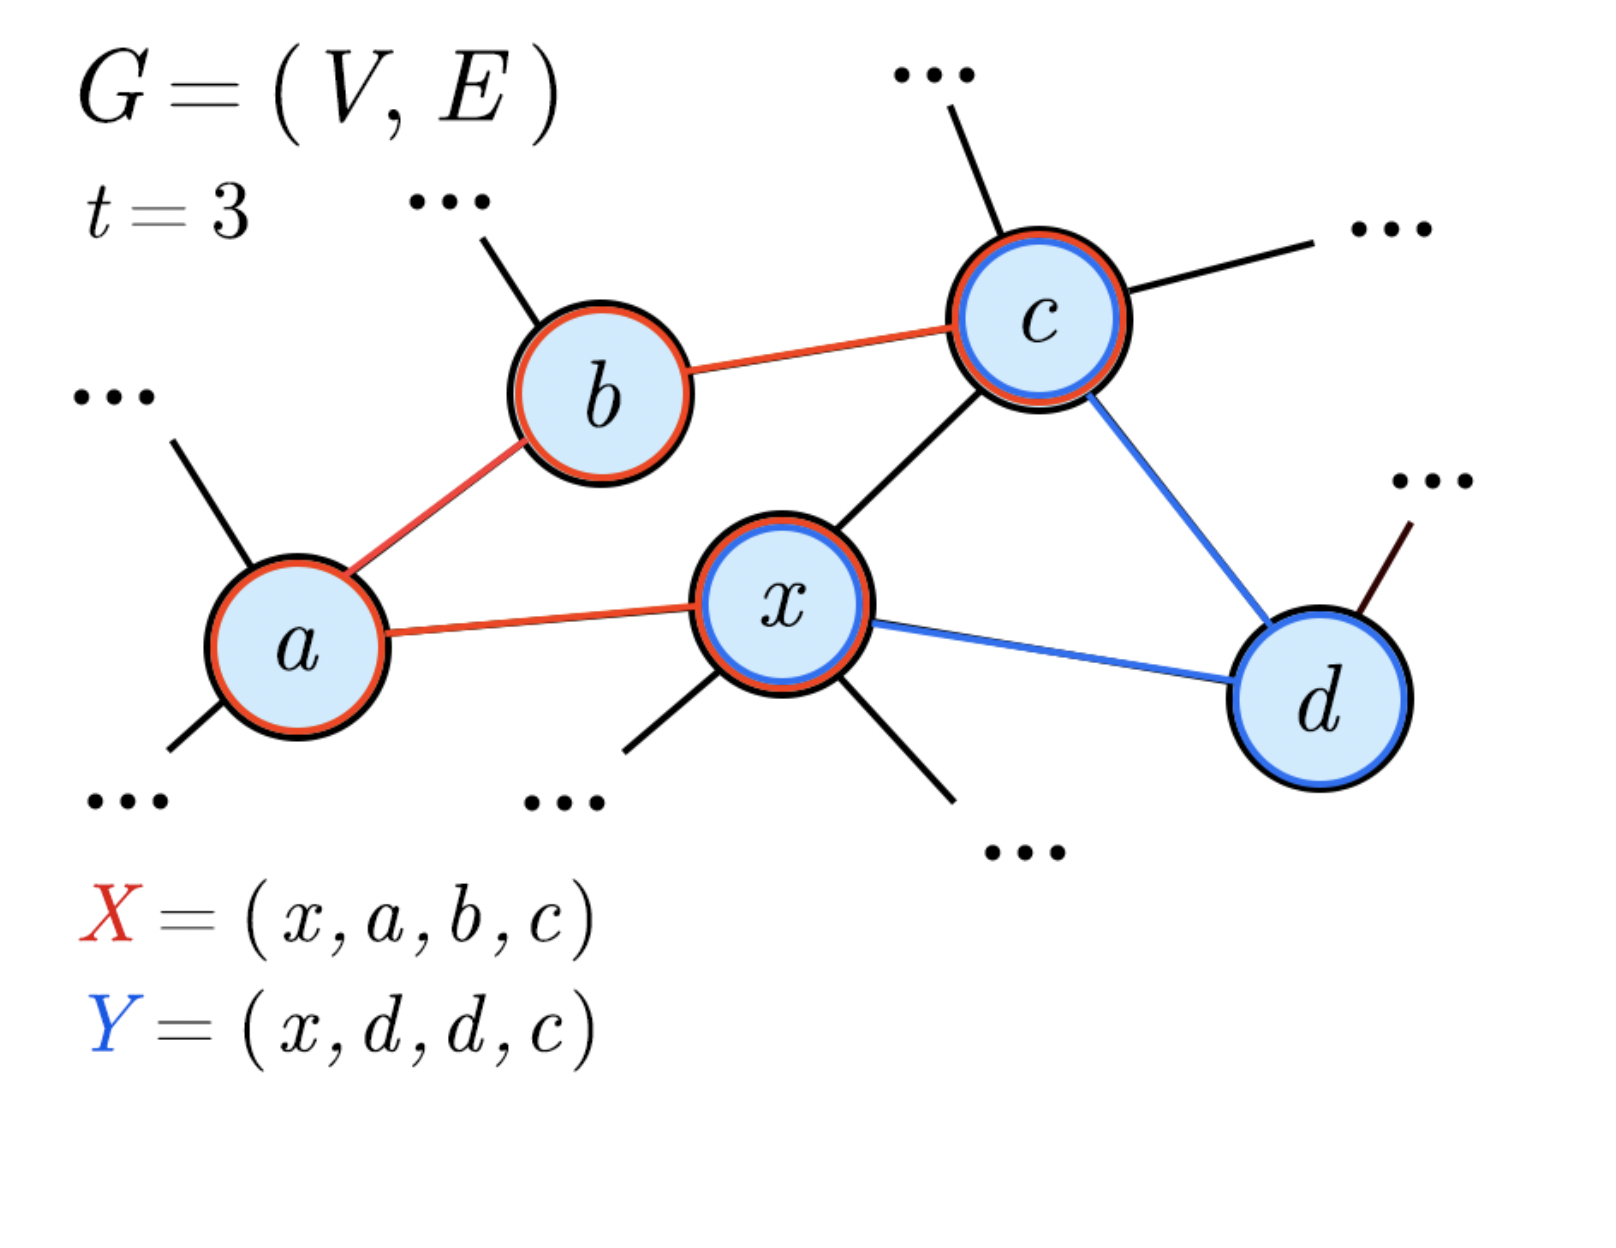
\includegraphics[trim={0 2cm 0 0}, clip, width=8cm]{diagrams/5.png}
\end{figure}
\end{frame}

\begin{frame}
\frametitle{Objective and Related Work}
\textbf{Goal:} Measuring intersections of multiple random walks gives a heuristic for estimating graph parameters ($m$, $n$) accurately and efficiently (in as few time-steps as possible).\medskip
\begin{itemize}
    \item In the above example, we would measure pairs of times $(t,s)$ such that $X_t=Y_s$.
    \item Possible applications: Surveying social networks, dealing with graphs too large for direct manipulation.
\end{itemize}\medskip
Builds on recent work by the authors and others that investigated related methods (recording return times to the start vertex) or other properties (spectral gap), while improving time bounds (at least $O(n)\to$ possibly sublinear).
\end{frame}

\subsection{Terminology and Main Ideas}

\begin{frame}
\frametitle{Recording \textsc{lrw} Data}
Fix some arbitrary vertex $x$. We consider the first $t$ time-steps of $K$ independent \textsc{lrw}s starting from $x$, $\textbf{X}^{(1)}_t,\dots,\textbf{X}^{(K)}_t$.\medskip 

Given a vertex sequence $\mathbf{v}=(v_1,\dots,v_t)$, let $r$ be the function replacing each vertex with the index of its first appearance.
\begin{itemize}
    \item E.g. $r:(g,a,a,c,g)\mapsto (1,2,2,3,1)$.
    \item This lets us assign numbers to vertices that are invariant under vertex-relabeling. 
\end{itemize}\medskip

Let $\Phi$ be the \textbf{profile} of such a sequence, defined by $\Phi(\mathbf{v})=(r(\mathbf{v}),(\deg(v_i))_{1\leq i\leq t})$.
\end{frame}

\begin{frame}
\frametitle{Desired Estimators}
We estimate some property of $G$, $\gamma(G)$ by 
    \[\hat{\gamma}_{K,t}=\textsc{est}\left(\Phi\left(\textbf{X}^{(1)}_t,\dots,\textbf{X}^{(K)}_t\right)\right).\]
Set $\epsilon>0$. Let $K$ be fixed depending on $\epsilon$. We will minimize $t(\epsilon,G)$ such that for $t\geq t(\epsilon,G)$, 
    \[\Prob\left(\left|\frac{\hat{\gamma}_{K,t}}{\gamma(G)}-1\right|>\frac{1}{2}\right)\leq \epsilon.\]
In other words, the paper gives algorithms with upper bounds on $t(\epsilon,G)$, depending on the parameter of interest.
\end{frame}

\begin{frame}
\frametitle{Definitions}
Let $P$ be the transition matrix for a $\textsc{lrw}$ on $G$.
\begin{itemize}
    \item \textbf{Fact:} \textsc{lrw}s converge to a stationary distribution $\pi$ given by $\pi(v)=\frac{\deg(v)}{2m}$.
    \item \textbf{Definition:} The \textbf{uniform mixing time} is 
    \[t_{\text{unif}}=\inf\left(t\geq 0:\max_{x,y\in V}\left|\frac{P^t_{xy}}{\pi(y)}-1\right|\leq \frac{1}{4}\right).\]
    \item \textbf{Definition:} The \textbf{relaxation time} is $t_{\text{rel}}=\left\lceil\frac{1}{1-\lambda_2}\right\rceil$, where $\lambda_2$ is the second-largest eigenvalue of $P$ (the largest one is $1$).
\end{itemize}
\end{frame}

\begin{frame}
\frametitle{Main Ideas}
$G$ has $n$ vertices and $m$ edges. Let its minimum degree be $d$.
\begin{itemize}
    \item If $G$ is \textbf{regular} (all vertices have equal degree), we can estimate $n$ in $O(t_{\text{rel}}^{3/4}\sqrt{n})$ steps.
    \item In arbitrary graphs, we can estimate $m$ in $O\left(t_{\text{rel}}^{3/4}\sqrt{\frac{m}{d}}\wedge \left(t_{\text{unif}}+t_{\text{rel}}^{5/6}\sqrt{n}\right)\right)$ steps, and estimate $n$ in an additional $O\left(t_{\text{unif}}\frac{m}{n}\right)$ steps. These bounds are optimal.
    \item These algorithms are not \textbf{self-stopping} (stop at some random time according to current information). This is unavoidable. If $m$ or a bound on the mixing time is known, however, there are self-stopping algorithms to estimate the other parameter.
\end{itemize}
\end{frame}

\subsection{Facts About Random Walks}
\begin{frame}
\frametitle{Intersections of \textsc{lrw}s}
Let $X,Y$ be independent \textsc{lrw}s. 
\begin{itemize}
    \item The \textbf{number of intersections} is $I_t=\sum_{i,j=0}^{t-1} \ind(X_i=Y_j)$. 
    \item The \textbf{weighted number of intersections} is $\mathcal{I}_t=\sum_{i,j=0}^{t-1} \ind(X_i=Y_j)$. \item The weighted number of intersections after the mixing time is $\mathcal{J}_t=\sum_{i,j=t_{\text{unif}}}^{t_{\text{unif}}+t-1} \ind(X_i=Y_j)$.
\end{itemize}
If $X$ starts from $x$, let $g_t(x,u)=\sum_{i=0}^{t-1} P^i(x,u)$ be the expected number of visits to $u$ before time $t$. It has been shown that 
\[\E_x\mathcal{I}_t = \sum_{u\in V}\frac{g_t(x,u)^2}{\deg(u)}=\sum_{i,j=0}^{t-1} \frac{P^{i+j}(x,x)}{\deg(x)}.\]
\end{frame}

\begin{frame}
\frametitle{Proposition 1}
\textbf{Bound} $\mathcal{I}_t$: For all vertices $x$, $\frac{t^2}{2m}\leq \E_x\mathcal{I}_t\leq \frac{t^2}{2m}+\frac{16t_{\text{rel}}^{3/2}}{d}$ and $\E_x\mathcal{I}_t^2\leq 4\left(\max_{a\in V} \E_a\mathcal{I}_t\right)\E_x \mathcal{I}_t$. Sketch:
\begin{itemize}
    \item Rewrite $\E_x\mathcal{I}_t=\frac{t^2}{m}+\frac{1}{2m}\sum_{i,j=0}^{t-1}\left(\frac{P^{i+j}(x,x)}{\pi(x)}-1\right)$.
    \item The sum is bounded by $\sum_{s=0}^\infty (s+1)\left(\frac{P^s(x,x)}{\pi(x)}-1\right)$. Technical arguments bound this by $\frac{t_{\text{rel}}}{(1-1/e)^2} \frac{g_{t_{\text{rel}}}(x,x)}{\pi(x)}$. 
    \item $g_t(x,x)$ and $t_{\text{rel}}$ can also be bounded.
    \item $\E_x\mathcal{I}_t^2=\sum_{u,v} \frac{1}{\deg(u)\deg(v)}\left(\sum_{i,k=0}^{t-1}\Prob_x(X_i=u,X_k=v)\right)$. The bound follows by working with the probabilities in terms of $g_t$s, then rewriting in terms of $\E_u\mathcal{I}_t$ and $\E_x\mathcal{I}_t$.
\end{itemize}

\end{frame}

\begin{frame}
\frametitle{Proposition 2}
\textbf{Bound} $\mathcal{J}_t$: For all vertices $x$, $\left(\frac{3}{4}\right)^2 \frac{t^2}{2m}\leq \E_x\mathcal{J}_t\leq \left(\frac{5}{4}\right)^2 \frac{t^2}{2m}$ and $\E_x \mathcal{J}_t^2\lesssim \frac{t^2}{m^2}\left(t^2+nt_{\text{rel}}^{5/3}\right)$. Sketch:
\begin{itemize}
    \item $\E_x\mathcal{J}_t=\sum_{y,z} P^{t_{\text{unif}}}(x,y)P^{t_{\text{unif}}}(x,z)\E_{y,z}\mathcal{I}_t$. Approximate $P^{t_{\text{unif}}}$ by $\pi$. Then apply $\sum_{y,z} \pi(y)\pi(z)\E_{y,z}\mathcal{I}_t=\frac{t^2}{2m}$.
    \item Write $\E_x\mathcal{J}_t^2\lesssim \sum_{y,z} \pi(y)\pi(z)\E_{y,z}\mathcal{I}_t^2$.
    \item Writing $\E_{y,z}\mathcal{I}_t^2$ in terms of $g_t$s and applying reversibility gets the bound $\frac{t^2}{m^2}\sum_{i,j=0}^{t-1}\sum_u P^{i+j}(u,u)$. The technique from Prop. 1 and a bound on $\sum_u P^t(u,u)$ complete the proof.
\end{itemize}
\textbf{Corollary:} Given $X$, $Y$, if $\tau_I=\inf(t\geq 0: X_{0:t}\cap Y_{0:t}\neq \varnothing)$ is the time of the first intersection, $\max_{x,y\in V}\E_{x,y}\tau_I\lesssim t_{\text{rel}}^{3/4}\sqrt{m/d}$.
\end{frame}

%%%%%%%%%%

\section{Estimating Parameters}
\subsection{Estimating the Number of Edges}
\begin{frame}
\frametitle{Estimator 1}
Proposition 1 gives us a simple method for estimating the number of edges in general graphs. Recall that we derived
$$
\frac{t^2}{2m} \leq \E_x\mathcal{I}_t \leq \frac{t^2}{2m} + \frac{16t_{\text{rel}}^{3/2}}{d},
$$
where $m$ is the number of edges, $d$ is the minimum degree, and $t_{\text{rel}}$ is the relaxation time. If we replace $\E_x\mathcal{I}_t$ with its empirical average, this inequality suggests the estimator $\hat{m}_t$ given by
$$
\hat{m}_t = \frac{t^2}{\frac{2}{K}\sum_{k=1}^K \mathcal{I}_t^{(k)}}
$$
where each $\mathcal{I}_t^{(k)}$ is an independent copy of $\mathcal{I}_t$.
\end{frame}

\begin{frame}
\frametitle{Estimator 2}
Proposition 2 gives us a very similar method for estimating the number of edges in general graphs. Recall that we derived
$$
\left(\frac{3}{4}\right)^2\frac{t^2}{2m} \leq \E_x\mathcal{J}_t \leq \left(\frac{5}{4}\right)^2\frac{t^2}{2m}
$$
where $m$ is the number of edges, $d$ is the minimum degree, and $t_{\text{rel}}$ is the relaxation time. If we replace $\E_x\mathcal{J}_t$ with its empirical average, this inequality suggests the estimator $\tilde{m}_t$ given by
$$
\tilde{m}_t = \frac{t^2}{\frac{2}{K}\sum_{k=1}^K \mathcal{J}_t^{(k)}}
$$
where each $\mathcal{J}_t^{(k)}$ is an independent copy of $\mathcal{J}_t$.
\end{frame}

\begin{frame}
\frametitle{Guarantees on these Estimators}
Using Propositions 1 and 2, we can derive some guarantees on these estimators. For $\hat{m}$, if we have $t\geq 4\sqrt{3}t_{\text{rel}}^{3/4}\sqrt{m/d}$, then we can show using a Chebyshev bound that
$$
P\left(\left|\frac{\hat{m}_t}{m} - 1\right| > \frac{1}{2}\right) = O\left(\frac{1}{K}\right),
$$
and for $\tilde{m}$, if we have $t\gtrsim t_{\text{rel}}^{5/6}\sqrt{n}$, then once again we obtain
$$
P\left(\left|\frac{\tilde{m}_t}{m} - 1\right| > \frac{1}{2}\right) = O\left(\frac{1}{K}\right).
$$
\end{frame}

\begin{frame}
\frametitle{When do we Achieve this Bound?}
On what sorts of graphs do we absolutely require that $t\gtrsim t_{\text{rel}}^{5/6}\sqrt{n}$? Consider the graph generated as follows, for $k,q\geq 1$:
\begin{itemize}
    \item Start with a 3-regular graph on $k$ vertices.
    \item Replace each node with a clique (fully-connected subgraph) with $q$ nodes.
    \item Replace each edge with a path of length $q$.
\end{itemize}
\end{frame}

\begin{frame}
\frametitle{When do we Achieve this Bound?}
Here is an example of such a graph, where each $K_q$ denotes a clique with $q$ nodes.
\[
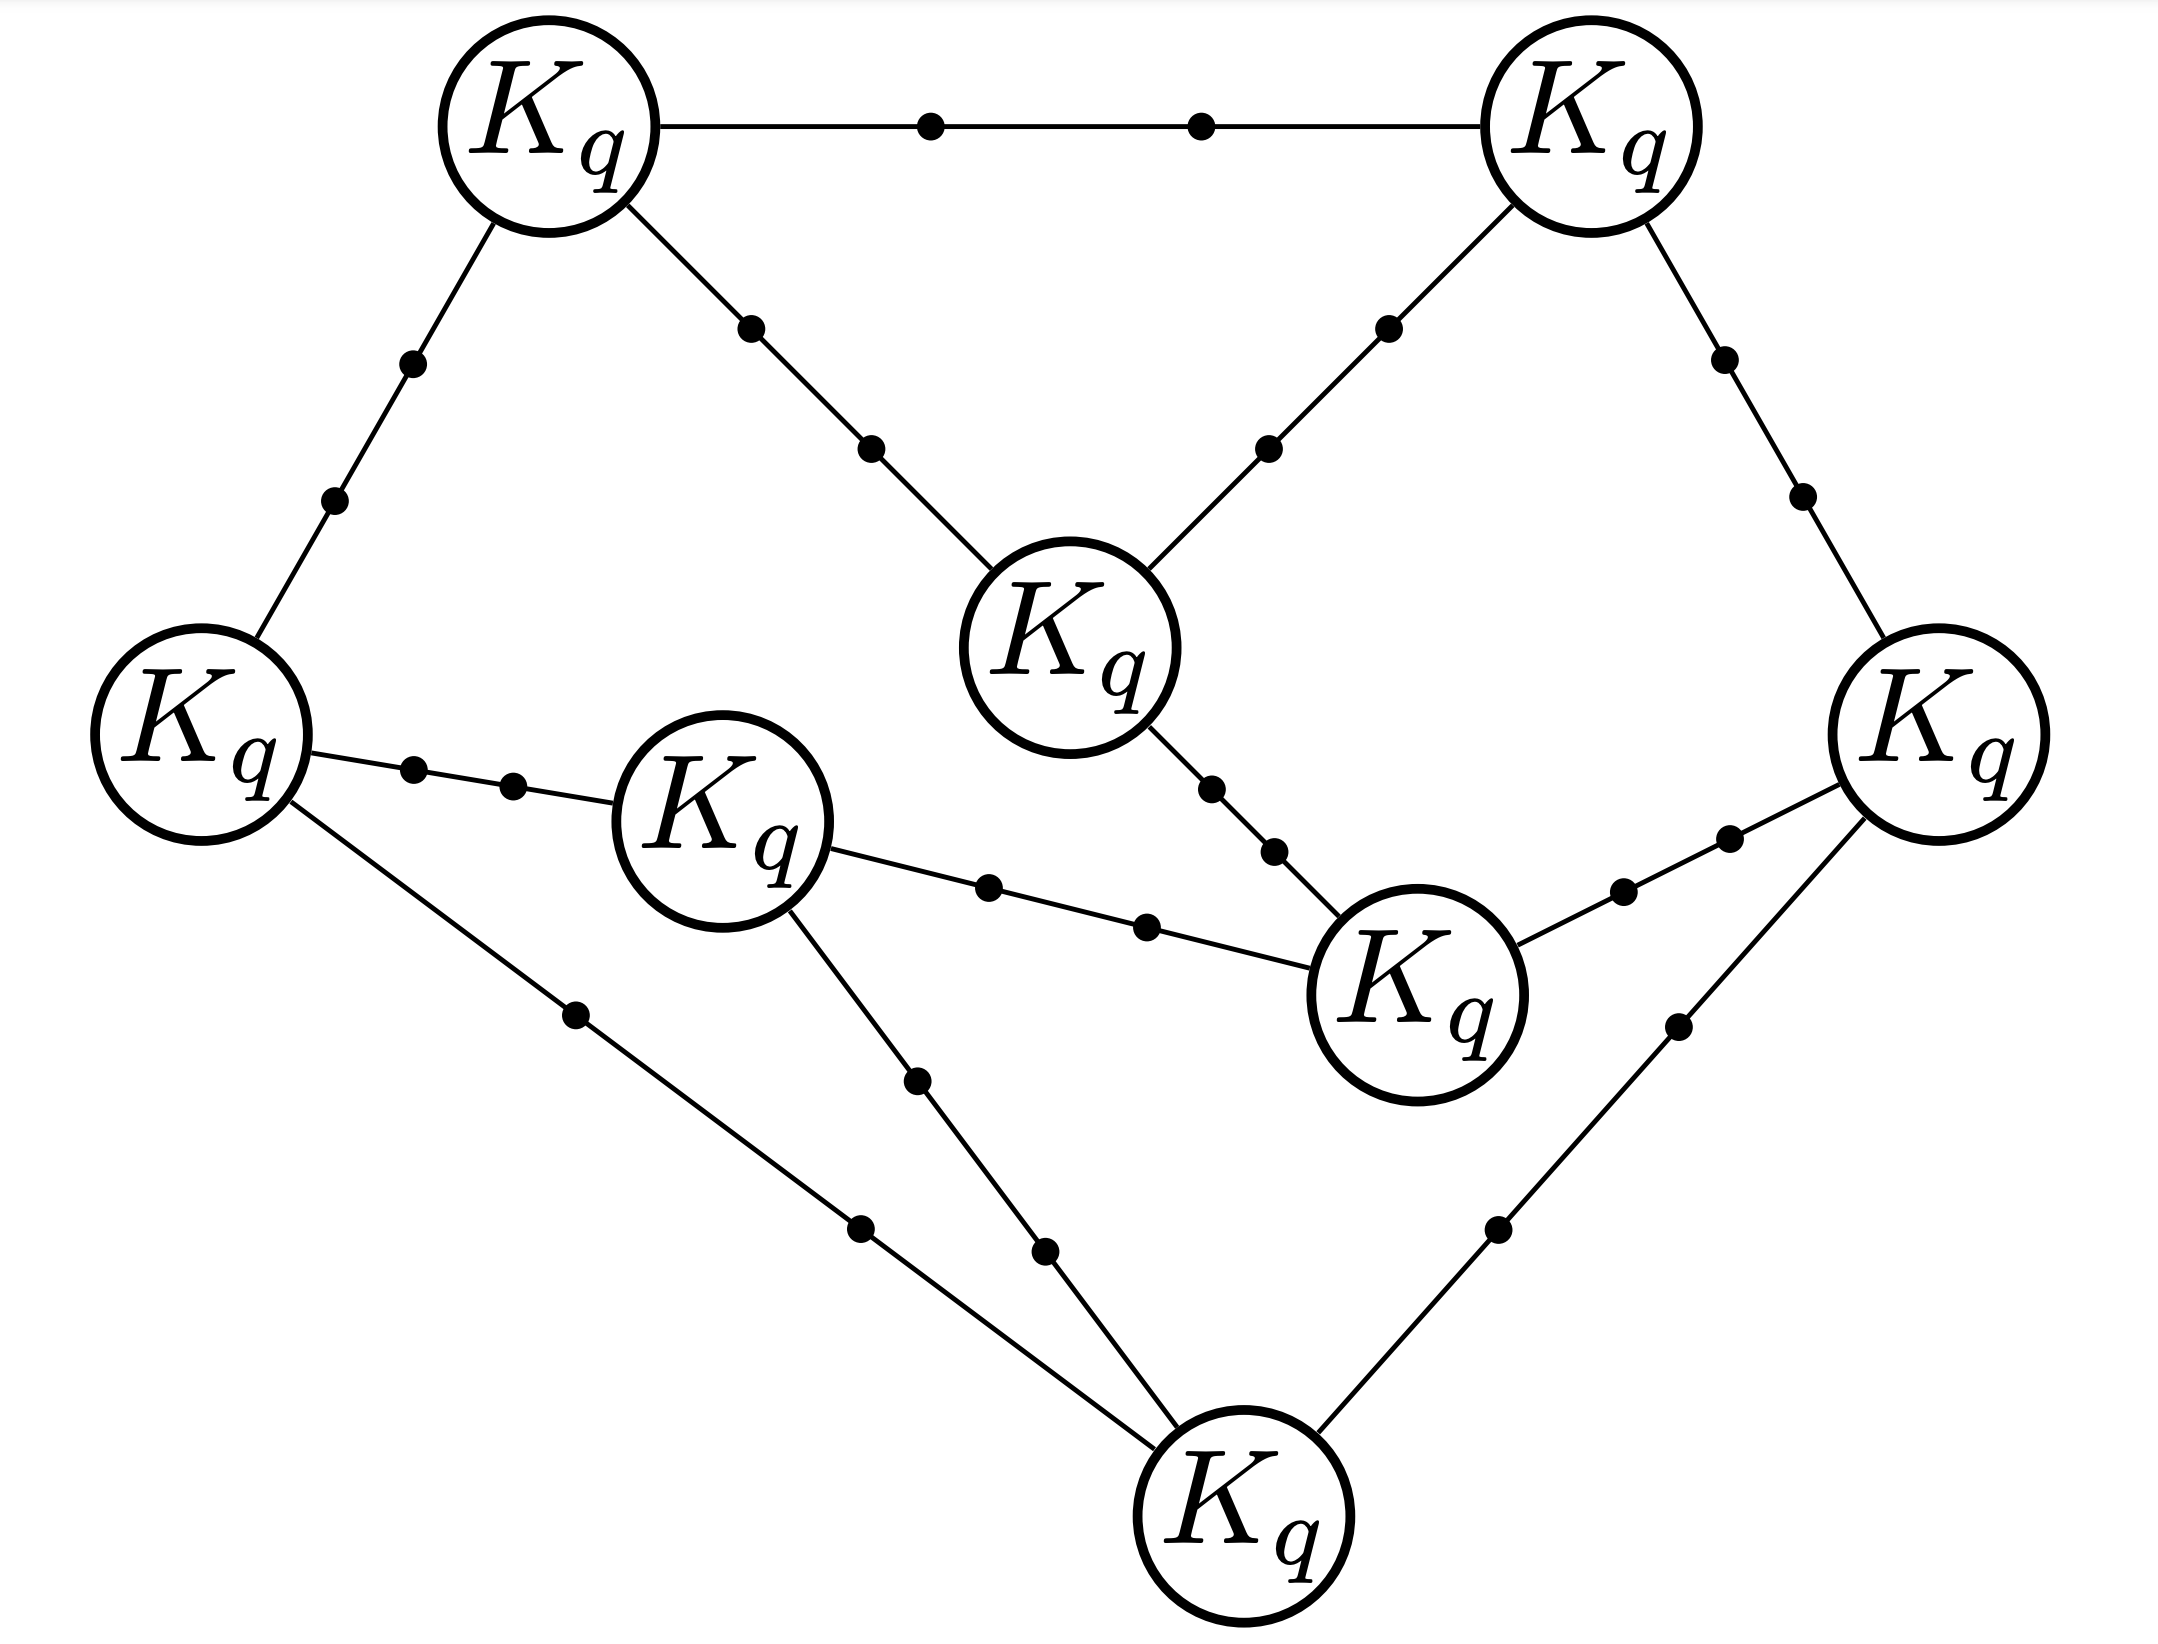
\includegraphics[width=2.5in]{diagrams/graf.png}
\]
\end{frame}

\begin{frame}
\frametitle{When do we Achieve this Bound?}
We can compute that this graph satisfies $n\sim kq$ and $t_{\text{rel}} \sim q^3$. Sketch of the proof:
\begin{itemize}
    \item To estimate the number of edges, we need to estimate the order of $k$.
    \item We can show that for a regular 3-graph on $k$ vertices, the time it takes a l.r.w. to make a cycle (which allows us to distinguish such a graph from an infinite tree) is of order $\sqrt{k}$.
    \item Adding the cliques and chains increases the amount of time to make a cycle to $\sim q^3\sqrt{k} \sim t_{\text{rel}}^{5/6}\sqrt{n}$.
\end{itemize}
\end{frame}

\subsection{Estimating the Number of Vertices}
\begin{frame}
\frametitle{Regular Graphs}
For a regular graph with $n$ nodes of degree $d\geq 1$, Proposition 1 simplifies to
$$
\frac{t^2}{n} \leq \E_x I_t \leq \frac{t^2}{n} + 16t_{\text{rel}}^{3/2},
$$
implying the estimator
$$
\hat{n}_t = \frac{t^2}{\frac{1}{K}\sum_{k=1}^K I_t^{(k)}}
$$
where each $I_t^{(k)}$ is an independent copy of $I_t$. Note that once again, we've simply replaced $\E_x I_t$ with its empirical average.
\end{frame}

\begin{frame}
\frametitle{Guarantees on this Estimator}
Using Proposition 1, if we have $t\geq 2\sqrt{6}t_{\text{rel}}^{3/4}\sqrt{n}$, then we can show that
$$
P\left(\left|\frac{\hat{n}_t}{n} - 1\right| > \frac{1}{2}\right) = O\left(\frac{1}{K}\right).
$$
\end{frame}

\begin{frame}
\frametitle{When do we Achieve this Bound?}
We require that $t\gtrsim t_{\text{rel}} \sqrt{n}$ on a cyclic graph on $n$ vertices. Here, we can compute that $t_{\text{rel}}\sim n^2$, so $t_{\text{rel}}^{3/4}\sqrt{n}\sim n^2$. Any random walk procedure needs $n^2$ steps to distinguish a cycle of size $n$ from a cycle of size $2n$.

\medskip

We may also find regular graphs that achieve this bound when we vary $t_{\text{rel}}$ and $\sqrt{n}$ \textit{independently}.

\medskip

For general graphs, we can show that $t\gtrsim t_{\text{rel}}^{5/6}\sqrt{n}$, the bound we used to estimate the number of edges, is insufficient. However, it is easy to derive a bound on the number of vertices given the number of edges.
\end{frame}

\section{Additional Algorithms}
\subsection{Self-Stopping Algorithms}
\begin{frame}
\frametitle{No sub-linear time self-stopping algorithms}

Suppose we don't know the size of the graph and update our estimator $\Est(\Phi(X_0^t))$ as we observe the step $t$ of our random walks. Based on the result, can we construct a stopping function $\Stop$ and an estimating function $\Est$ st. for all graphs $G$ and $x\in V(G)$
\[
\Prob_x\left(\{T<\delta n_G\}\cap \left\{|\frac{\Est(\Phi(X_0^\tau))}{n_G}-1|\leq \frac12\right\}\right)>\frac34
\]
where $\tau = \inf \{t\ |\ \Stop(t) = 1\}$?

\end{frame}

\begin{frame}
\frametitle{No sub-linear time self-stopping algorithms}

No sub-linear stopping time even if graph has nice properties (eg. $G$ is 3-regular, has $t_{\text{unif}}(G)\leq (\log n_G)^3$). 

Proof sketch:
\begin{itemize}
    \item Starting with graph $G$, construct graph $G^*$ by starting with $2^n$ copies of $G$, and connecting three random vertices of each copy $i$ to some other copy $j$ iff there exists an edge between $i$ and $j$ in another 3-regular graph $F$.
    \item Find coupled random walks $(X,Y)$ on $G$ and $G^*$, st. the probability the walks coincide up to time $\delta n$ exceeds 2/3
    \item Then applying our stopping and estimation function to both walks, the stopping time is the same, and the estimation at time $\tau$ is the same, but cannot be accurate with high probability for both graphs
\end{itemize}

\end{frame}

\begin{frame}
\frametitle{Self-stopping algorithm w/ upper bound on relaxation time}

With an upper bound $\tau$ on the relaxation time, for any $\eps$, we can estimate the number of edges st. $P(m<\hat{m}<38m) > 1-\eps$.

\begin{itemize}
\item Start with $q=0$, and guess $\hat{m}=2^q$. Let $t = \tau^{\frac34}\sqrt{2\hat{m}}$. 

\item Repeat $R = \ceil{8\log (4/\eps)+16\log(q+1)}$ times: considering $2K$ independent random walks, let $\mathcal{Q}_t$ be the average number of intersections up to time $t$, and call the experiment a success if $\mathcal{Q}_t\geq 18\tau^{\frac32}$. 

\item Stop if the number of successes exceeds $R/2$ (otherwise increment $q$).

\end{itemize}

\end{frame}

\begin{frame}
\frametitle{Self-stopping algorithm w/ upper bound on relaxation time}

From earlier, we have
\[
\tau^{\frac32}\frac{\hat{m}}{m}\leq \E[\mathcal{Q}_t]\leq \tau^{\frac32}\frac{\hat{m}}{m}+16\tau^{\frac32}
\]

\begin{itemize}
    \item If $\hat{m}<m$, then by Chebyshev, since $\E[\mathcal{Q}_t]\leq 17\tau^{\frac32}$, the probability of success is less than $\frac{\Var \mathcal{I}_t}{K\tau^3}$. With $K$ and $R$ large enough, the probability of $R/2$ successes on any trial where $\hat{m}<m$ is less than $\frac12\eps$.
    \item If $\hat{m}>19m$, then by Chebyshev, since $\E[\mathcal{Q}_t]> 19\tau^{\frac32}$, the probability of failure is less than $\frac{\Var \mathcal{I}_t}{K(\E[\mathcal{I}_t)^2]}$. With $K$ and $R$ large enough, the probability of fewer than $R/2$ successes on this trial is less than $\frac12\eps$.
\end{itemize}

\end{frame}

\subsection{Estimating the mixing time}
\begin{frame}
\frametitle{Defining the mixing time from a vertex}

If $\pi(y)$ is the stationary distribution, define the following $\ell^2$ measure of distance
\[
\delta_x(t) = \sqrt{\sum_y \pi(y)\cdot (\frac{\Prob(X_t = y)}{\pi(y)}-1)^2}
\]

We want to estimate, the mixing time from some vertex $x$, ie. for some $\delta\in (0,1)$,
\[
t_x(\delta) := \inf \{t\ |\ \delta_x(t)^2<\delta \}
\]

\end{frame}

\begin{frame}
\frametitle{Estimating the mixing time from a vertex}

If we know $m$, for any $\eps$, we can estimate the mixing time from a vertex $t_x(\delta)$ st. $P(\frac12t_x(\delta)<\hat{t}<2t_x(\frac14\delta)>1-\eps$.

\begin{itemize}
\item Start with $q=0$, and guess $\hat{t}=2^q$. Let $K = \ceil{K\delta^{-2}\ceil{\sqrt{m}t^{-1/4}}}$. 

\item Repeat $R = \ceil{8\log (4/\eps)+16\log(q+1)}$ times: considering $K$ independent random walks, let $\mathcal{L}_t$ be the average number of intersections of any two walks between times $t$ and $2t-1$, and call the experiment a success if $\mathcal{L}_t<(1+\delta/2)\cdot \frac{t^2}{2m}$. 

\item Stop if the number of successes exceeds $R/2$ (otherwise increment $q$).

\end{itemize}

\end{frame}

\begin{frame}
\frametitle{Estimating the mixing time from a vertex}

The proof uses the following lemma: if $X,Y,Z$ independent random walks and $\mathcal{L}_t^{(X,Y)}$ is the number of intersections of $X$ and $Y$ from time $t$ to $2t$, then $\E\mathcal{L}^{(X,Y)}_t = \sum_{i,j=t}^{2t-1}\frac1{2m}\cdot (d_x(\frac{i+j}2)^2 +1)$\bigskip\\

The algorithm terminates in expected time
\[
O(\delta^{-2}\sqrt{m}t_x(\delta/4)^{\frac34}\log\log t_x(\delta/4))
\]

A good estimate on the number of edges is enough to make the algorithm work
\end{frame}

\begin{frame}
\frametitle{Works Cited}
\begin{itemize}
    \item Ben-Hamou, A., Oliveira, R., Peres, Y. (2018). \textit{Estimating Graph Parameters with Random Walks.} arXiv:1709.00869.
    \item Oliveira, R. I., Peres, Y. (2018). \textit{Random walks on graphs: new bounds on hitting, meeting, coalescing and returning.} arXiv:1807.06858.
    \item Ben-Hamou, A., Oliveira, R., Peres, Y. (2018). \textit{Estimating graph parameters via random walks with restarts.} doi.org/10.1137/1.9781611975031.111.
\end{itemize}
\end{frame}

\end{document}
